\section{Półklasyczna teoria przewodnictwa elektronowego metali}
\subsection{Zdegenerowany gaz elektronowy}
 \subsubsection{Wstęp}
 W 1926 roku Pauli opublikował zakaz Pauliego, a Fermi i Dirac- statystyki dla elektronów. Statystyki są zupełnie inne od tych, które założył Drude (w statystykach Fermiego-Diraca elektrony mają prędkość zgodnie z rozkładem Maxwella).\\
 W 1927 roku Sommerfeld zmodyfikował teorię Drudego, zakładając w nim statystykę Fermiego- Diraca. Jest to tzw. półklasyczna (a nie kwantowa) teoria, ponieważ Sommerfeld założył kwantową statystykę Fermiego-Diraca, w sposób kwantowy opisał również prawdopodobieństwo przejść, natomiast cały aparat matematyczny pozostał klasyczny.
\subsubsection{Zakaz Pauliego}
\begin{enumerate}
\item \textbf{Tw.} Zakaz Pauliego\\ Prawdopodobieństwo znalezienia w układzie \emph{jednorodnych i nieoddziałujących} fermionów pary cząstek o jednakowych liczbach kwantowych jest równe 0.\\
 \item Komentarz:
\begin{itemize}
\item \emph{nieoddziałujących}- bo jest to gaz elektronowy. Zakładamy, że jest tak rzadki, że nie ma w nim zderzeń elektron-elektron. Są za to zderzenia elektron-jon (jest to zatem gaz Lorentza).
\item\emph{ jednakowych}- nie możemy rozróżnić elektronów- bo zgodnie z mechaniką kwantową nie możemy określić dokładnie ich trajektorii.\\
Przykład: Rozważmy 2 cząstki. O ile w pierwszej chwili możemy określić ich położenie (są to dwa gaussiany; patrz- rysunek poniżej), to w następnych chwilach   ich rozkłady się przekrywają i nie jesteśmy w stanie ustalić położenia danej cząstki - stąd nie możemy określić trajektorii żadnej z tych cząstek.\\
Ewolucję czasową tych 2 cząstek przedstawia poniższy rysunek.
\begin{center}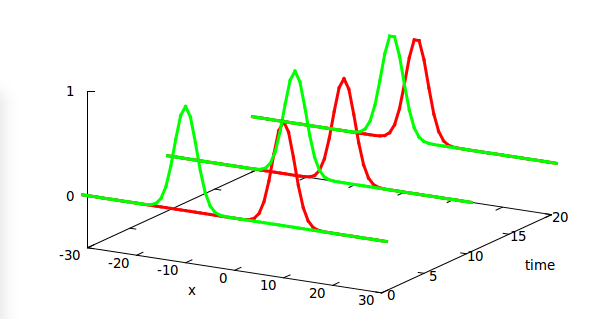
\includegraphics[scale=0.75]{obrazki/wykl_7_obrazek_1.png}\end{center}
To powoduje, że gaz ten nie jest już klasyczny. Jest to tzw. gaz zdegenerowany.
\end{itemize}
\end{enumerate}

\subsubsection{Stan układu- liczby kwantowe}
\begin{itemize}
\item Stan układu
Klasyczny stan układu jest określony przez:
\begin{equation} |\r,\p\left>z\end{equation}
Kwantowy stan układu jest określony przez:
\begin{equation} |\Psi\left>\end{equation}
\item Pęd jako liczba kwantowa
gdzie $\Psi$ to abstrakcyjny wektor stanu.\\
Funkcja falowa przedstawia się wzorem:
\begin{equation}\Psi_{\p}\arg=\frac{1}{V}e^{-\frac{i}{\hbar}(E(\p)t-\p\cdot\r)}\end{equation}
gdzie $\p$ jest liczbą kwantową, bo jednoznacznie określa funkcję falową. Można zatem oznaczać:
\begin{equation} \Psi_{\p}\arg=\right< \r|\Psi_{\p(t)}\left>=\right< \r|\p\left>\end{equation}
gdzie $|\Psi_{\p(t)}\left>$ to wektor stanu zapisany w obrazie Schroedingera.\\
\item Spin jako liczba kwantowa
Kolejną liczbą kwantową jest rzut spinu $\sigma$. Można zatem zapisać:
\begin{equation}|\Psi\left>=|\p,\sigma\left>\end{equation}
\end{itemize}
\subsubsection{Poziomy energetyczne}
Relacja de Broglie'a przedstawia:
\begin{equation}\p=\hbar\ka\end{equation}
gdzie k jest dyskretne:
\begin{itemize}
\item sztywne warunki brzegowe:
\begin{equation} k_i=\frac{n_i\pi}{L_i}~~~~;n_i\epsilon\mathbb{N}\end{equation}
\item periodyczne warunki brzegowe
\begin{equation} k_i=\frac{2n_i\pi}{L_i}~~~~;n_i\epsilon\mathbb{Z}\end{equation}
\end{itemize}
Warunki te przedstawia schematycznie poniższy rysunek:
\begin{center}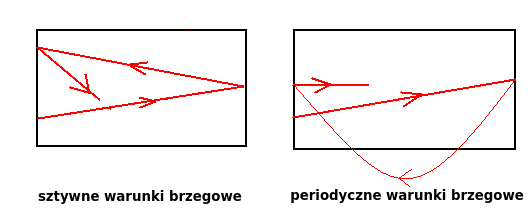
\includegraphics[scale=0.75]{obrazki/wykl_7_obrazek2.png}\end{center}
Z kolei relacja dyspersji dla elektronów swobodnych określa się wzorem:
\begin{equation}E=\frac{p^2}{2m}=\frac{\hbar^2\ka^2}{3m}\end{equation}
Skoro k jest dyskretne, to również E jest dyskretne. Oznacza to, że energia jest skwantowana, czyli istnieją poziomy matematyczne, pokazane na poniższym rysunku.
\begin{center}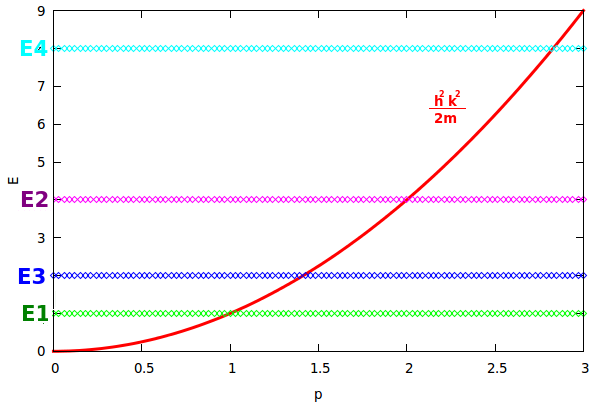
\includegraphics[scale=0.5]{obrazki/wykl_7_obrazek3.png}\end{center}
\subsubsection{Rozkład Fermiego-Diraca}
\begin{enumerate}
\item Tw. Dla niezerowej temperatury średnia liczba fermionów przypadających na 1 stan jest określony rozkładem Fermiego-Diraca:
\begin{equation} f_{FD}(\Ep)=f_{FD}(\p)=\frac{1}{1+e^{\frac{\Ep-\mu}{k_BT}}}\end{equation}
\item Asymptotyczne zachowanie:\\
1) W niskich temperaturach:
\begin{equation}\lim\limits_{T \to 0}f_{FD}(\Ep)=\theta(\Ep-\mu)= \begin{cases} 1~~\text{dla}~\Ep\right< \mu \\ 0~~\text{dla}~\Ep\left>\mu\end{cases}\end{equation}
gdzie $\theta$ to funkcja schodkowa Heavi-Side'a.\\
2) W wysokich temperaturach rzędu $|E-\mu|\left>\left>k_BT$:
\begin{equation}\lim\limits_{\frac{|E-\mu|}{k_BT}\rightarrow\infty} f_{FD}(\Ep)=e^{-\frac{\Ep-\mu}{k_BT}}=f_B(\Ep)\end{equation}
gdzie $f_B$ to rozkład Boltzmanna.\\
3) W punkcie $\Ep=\mu$:
\begin{equation}f_{FD}(\Ep=\mu)=\frac{1}{1+1}=\frac{1}{2}\end{equation}
\item Jak wyznaczyć potencjał chemiczny $\mu$?\\
a) Z równania:
\begin{equation} N=(2\sigma+1)\sum_{\p}f_{FD}(\Ep)\end{equation}
W ośrodku nieskończonym:
\begin{equation}V\rightarrow\infty:~~N=(2\sigma+1)\frac{V}{(2\pi\hbar)^3}\int d^3p f_{FD}(\Ep)\end{equation}
b) z równania na koncentrację\\
Pamiętamy, że koncentracja elektronów to:
\begin{equation}n=\frac{N}{V}\end{equation}
gdzie V to objętość naczynia, w którym są elektrony.\\
Zatem:
\begin{equation}n=N=\frac{2\sigma+1}{(2\pi\hbar)^3}\int d^3p f_{FD}(\Ep)=\frac{2\sigma+1}{(2\pi\hbar)^3}\int d^3p \frac{1}{1+e^{\frac{\frac{p^2}{2m}-\mu}{k_BT}}}\end{equation}
n można fizycznie zmierzyć w pomiarze efektu Halla.
\item Ogólny kształt funkcji rozkładu Fermiego-Diraca:
\begin{center}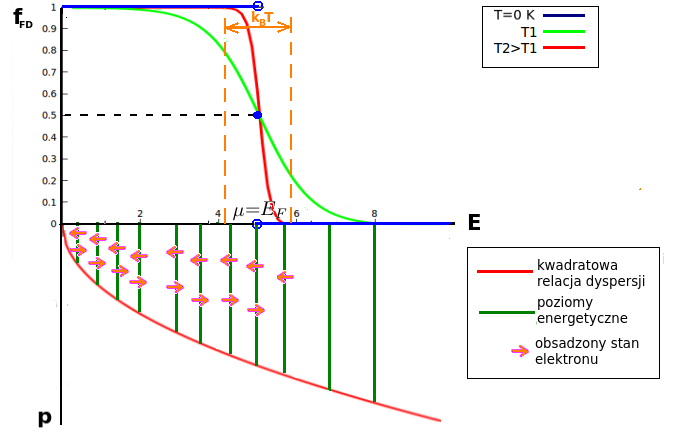
\includegraphics[scale=0.75]{obrazki/wykl_7_obrazek4.png}\end{center}
Zgodnie z zakazem Pauliego, na każdym poziomie energetycznym są maksymalnie 2 elektrony- o przeciwnych spinach.\\
Elektrony mogą przeskakiwać ze stanów obsadzonych do stanów nieobsadzonych w  okolicy Energii Fermiego, w przedziale o szerokości $k_BT$.
\item Pochodna funkcji rozkładu Fermiego Diraca:\\
W $T=0 K$:
\begin{equation}\frac{\partial f_{FD}(\Ep)}{\partial E}=-\delta(\Ep-E_F)\end{equation}
W $T\left>0 K$:
\begin{equation}\frac{\partial f_{FD}(\Ep)}{\partial E}=-\frac{1}{\pi}\frac{k_BT}{(\Ep-E_F)^2+(k_BT)^2}\end{equation}
Powyższy wyraz to Lorencjan. \\
Jest to tzw. funkcja spektralna.[NO I??????????????????? CO TO JEST??]
\begin{center}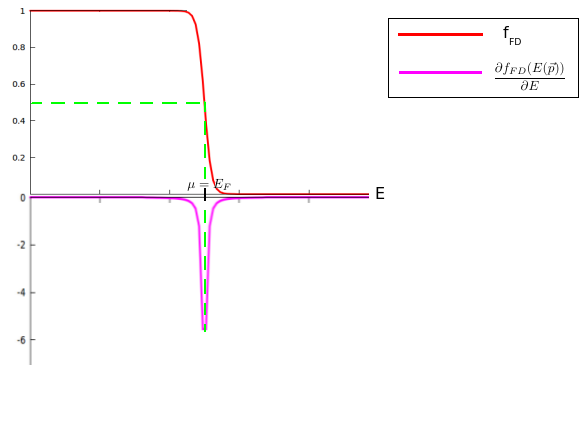
\includegraphics[scale=0.5]{obrazki/wykl_7_obrazek5.png}\end{center}
\end{enumerate}
\subsection{Całki zdarzeń $I[\f]$- przybliżenie czasu relaksacji (PCR)}
\subsubsection{Całka zdarzeń- definicja}
Uw. Aby uzyskać czytelność wzorów, dalej w indeksach pominięto wektor nad pędami: $\p\equiv p$.
\begin{equation}I[\f]=\sum_{p'}\{S_{p'p}-S_{pp'}\}\end{equation}
gdzie $\p'$ to pęd końcowy, natomiast:
\begin{equation}S_{pp'}=Q_{pp'}\f[1-\fp]\end{equation}
gdzie:\\
\begin{itemize}
\item Q opisuje szybkość przejść między $\p$ i $\p'$ (czyli szybkość rozproszeń);
\item$\f$ to stan, w którym jest elektron;
\item$\fp$ to stan, do którego elektron się rozprasza (na atomie).
\item$\r$ w obu wyrazach jest ten sam, czyli elektron rozprasza się w 1 punkcie przestrzeni (nie przemieszcza się w czasie rozproszenia).
\begin{center}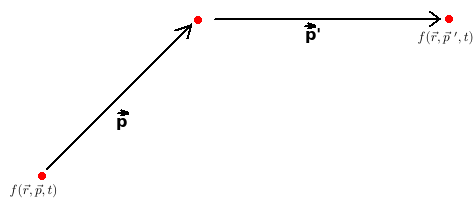
\includegraphics[scale=0.5]{obrazki/wykl_7_obrazek6.png}\end{center}
\end{itemize}
\subsubsection{Równanie Boltzmana- rozwiązanie}
\begin{enumerate}
\item Ogólna postać, z zastosowaniem definicji całki zdarzeń:
\begin{equation}\partial_t\f+\v\cdot\nab{r}\f+q(E+\v\times\B)\cdot\nabla_p\f=\end{equation}
\begin{equation} =\sum_{p'}\{Q_{p'p}\fp(1-\f)-Q_{pp'}\f(1-\fp\}\nonumber\end{equation}
\item Zasada równowagi mikroskopowej:\\
Szybkość przejścia ze stanu 1 do stanu 2 i szybkość przejścia ze stanu 2 do stanu 1 jest taka sama:
\begin{equation}Q_{p'p}=Q_{pp'}\end{equation}
\item Zatem całka zdarzeń:
\begin{equation}I[\f]=\sum_{p'}Q_{p'p}\{\fp-\fp\f-\f+\f\fp\}=\end{equation}
\begin{equation}=\sum_{p'}Q_{p'p}\{\fp-\f\}=\nonumber\end{equation}
\begin{equation}=-\f\sum_{p'}Q_{p'p}\{1-\frac{\fp}{\f}\}\nonumber\end{equation}
\item Wprowadzenie czasu relaksacji:\\
Wymiarem sumy obecnej w całce zdarzeń jest wymiar szybkości $Q_{p'p}$, czyli $\frac{1}{s}$. To jest przesłanka, by traktować tę sumę jako \textbf{odwrotność czasu relaksacji} $\tau$:
\begin{equation}\sum_{p'}Q_{p'p}\{1-\frac{\fp}{\f}\}\equiv=\tau^{-1}(\r,\p,t)\end{equation}
zatem: 
\begin{equation}I[\f]=-\frac{\f}{\tau(\r,\p,t)}\end{equation}
Wówczas równanie Boltzmana:
\begin{equation}\partial_t\f+\v\cdot\nab{r}\f+\underbrace{q(E+\v\times\B)}_{\text{siła Lorentza}~F_L}\cdot\nabla_p\f=-\frac{\f}{\tau(\r,\p,t)}\end{equation}
Wprowadza się również wyrażenie:
\begin{equation}\tau^{-1}(\p)=\sum_{p'}Q_{pp'}\end{equation}
które jest miarą siły oddziaływania z atomami (rozpraszania na nich).
Wówczas:
\begin{equation}I[\f]=\frac{\f}{\tau(\p)}-\sum_{p'}Q_{p'p}\fp=\end{equation}
\begin{equation}=\frac{\f-\frac{\sum_{p'}Q_{p'p}\fp}{\sum_{p'}Q_{p'p}}}{\tau(\p)}=\nonumber\end{equation}
\begin{equation}=\frac{\f-f_0(\r,\p,t)}{\tau(\p)}\nonumber\end{equation}
gdzie:
\begin{itemize}
\item $\f$ to nierównowagowa funkcja rozkładu
\item $f_0(\r,\p,t)$ to równowagowa funkcja rozkładu\\
\end{itemize}
Dla gazu elektronowego:
\begin{equation}f_0(\r,\p,t)=f_{FD}\end{equation}

\item Równanie Boltzmana zyskuje postać:
\begin{equation}\partial_t\f+\v\cdot\nab{r}\f+\vec{F}_L\cdot\nabla_p\f=-\frac{\f-f_0(\r,\p,t)}{\tau(\p)}\end{equation}
\item Założenia\\
\begin{itemize}
\item[I.] Badamy układy stacjonarne: $\f=f(\r,\p)$ - nie zależy od $t$
\item[II.] Układ jest jednorodny: $f(\r,\p)=f(\p)$ - nie zależy od $\r$
\end{itemize}
Założenia te wprowadzają idealny gaz elektronowy.
\item Zatem równanie Boltzmanna dla idealnego gazu elektronowego:
\begin{equation}q\E\cdot\nabla_{p}f(\p)=-\frac{f(\p)-f_0(\p)}{\tau(\p)}~~~~/\cdot\tau(\p)\end{equation}
Biorąc pod uwagę, że $q=-e$:
\begin{equation}e\tau(\p)\E\cdot\nabla_{p}f(\p)=f(\p)-f_0(\p)\end{equation}
Stąd:
\begin{equation}\underbrace{f(\p)}_{\text{funkcja nierównowagowa}} =\underbrace{f_0(\p)}_{\text{funkcja równowagowa}} +\underbrace{e\tau(\p)E\cdot\nabla_{p}f(\p)}_{\delta f}\label{f.nierownowagowa}\end{equation}
gdzie:\\
$\delta f$ to odchylenie od stanu równowagowego (bo $\nabla_{p}f$). Zakładamy, że zaburzenie to jest niewielkie:
\begin{equation}f_0(\p)\left>\left>\delta f(\p)\end{equation}
Powyższe równanie ma postać rozwinięcia w szereg Taylora do 1. wyrazu
\item Wniosek:\\
Jeśli przyłożymy małe pole $\E$, to obowiązuje przybliżenie czasu urojonego i funkcję rozkładu rozwija się w szereg Taylora do 1. wyrazu (bo wychylenie jest niewielkie).\\
\item Iteracyjne rozwiązywanie równania (\ref{f.nierownowagowa}):
\begin{equation}f_1(\p)=f_0(\p)+e\tau(\p)\E\cdot\nabla_{p}f_0(\p)
\simeq
f_0(\p+\underbrace{e\tau(\p)}_{\delta \p}\E) \end{equation}
Wniosek:
Zmiana pędu spowodowana włączeniem pola $\E$ przesuwa rozkład $f_{FD}$ o pewne $\delta p$:
\begin{center}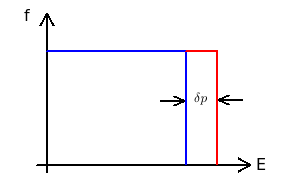
\includegraphics[scale=0.75]{obrazki/wykl_7_obrazek7.png}\end{center}
W książkach ta sama relacja jest pokazywana często w następujący sposób:
\begin{center}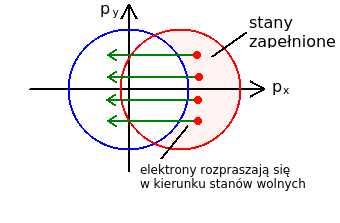
\includegraphics[scale=1]{obrazki/wykl_7_obrazek8.png}\end{center}
\item Gęstość prądu
Pamiętamy:
\begin{equation}\j=\sigma\E\end{equation}
Teraz możemy obliczyć:
\begin{equation}\j=evn=\frac{e}{(2\pi\hbar)^3}\int d^3p\v(\p)f(\p)=\end{equation}
\begin{equation}=\frac{e}{(2\pi\hbar)^3}\int d^3p\v(\p)\{f_0(\p)+e\tau(\p)\E\cdot\nabla_{p}f(\p)\}\nonumber\end{equation}
Funkcja równowagowa:
\begin{equation}f_0\propto p^2\end{equation}
opisuje pasma niebiorące udział w transporcie, zatem:
\begin{equation}\int d^3p\v f_0(\p)=0\end{equation}
Zatem:
\begin{equation}\j=\frac{e^2}{(2\pi\hbar)^3} \int d^3p\v(\p)\tau(\p)\nabla_{p}f(\p)\cdot\E\end{equation}
Ale:
\begin{equation} \nabla_p f(\p)=\frac{\partial E(\p)}{\partial p}\frac{\partial f(\Ep)}{\partial E}=\frac{\p}{m}\frac{\partial f}{\partial E}=\v \frac{\partial f}{\partial E}\end{equation}
Zatem: 
\begin{equation}\j=\underbrace{\frac{e^2}{(2\pi\hbar)^3} \int d^3p [\v(\p)\otimes\v(\p)]\tau(\p)\frac{\partial f}{\partial E}}_{\sigma}\E\end{equation}
\end{enumerate}

\end{document}
